\documentclass{article}

\usepackage[utf8]{inputenc}

% Packages
\usepackage{amsmath,amssymb}
\usepackage{bm}% boldmath
\usepackage{listings} % Code block (source code) \begin{lstlisting} 
\usepackage{natbib}
\usepackage{graphicx}
\usepackage{lmodern}
\usepackage[usenames,dvipsnames,svgnames,table]{xcolor}
\usepackage[textwidth=16cm,textheight=23cm]{geometry}

%\usepackage{inconsolata} % New monospace font

% URL
\usepackage{url}
\usepackage[colorlinks=true, a4paper=true, pdfstartview=FitV, linkcolor=blue, citecolor=blue, urlcolor=blue]{hyperref}

% Figures
\usepackage[font=small, labelfont=bf]{caption}
\usepackage{subfig} % Subfigures. Uses \subfloat[captions text]{figure}

% Tables
\usepackage{booktabs}   % Allows the use of \toprule, \midrule and \bottomrule in tables for horizontal lines
\newcommand{\ra}[1]{\renewcommand{\arraystretch}{#1}} % spaces in tables

% Itemize
\usepackage{enumitem}

% Commands
%\newcommand{\code}[1]{\texttt{#1}} % \code{inline code}
\newcommand{\code}[1]{{\small\ttfamily #1}} % \code{inline code}
\newcommand{\expval}[1]{\langle #1 \rangle} %
\renewcommand{\theequation}{\arabic{section}.\arabic{equation}} % Book format equation
\renewcommand{\thefigure}{\arabic{section}.\arabic{figure}} % Book format figure
\renewcommand{\vec}[1]{{\bf #1}} % Lars likes this better than arrow

% Set page attribution
\setlength{\parindent}{0pt}


% PSTRICKS
\usepackage{pstricks,pst-node,pst-tree} % includes graph additions
\usepackage{pst-pdf} % Compiles the pictures
\usepackage{pst-node}
\usepackage{pst-plot}
\usepackage{pst-3dplot}
%\usepackage{pstricks-add,babel}




\lstset{
language=Python,                        % Code langugage
commentstyle=\color{gray},              % Comments font
basicstyle=\small\ttfamily,             % Code font, Examples: \footnotesize, \ttfamily
keywordstyle=\bfseries\color{blue},
stringstyle=\color{orange},
numbers=left,                           % Line nums position
numberstyle=\tiny,                      % Line-numbers fonts
stepnumber=1,                           % Step between two line-numbers
numbersep=5pt,                          % How far are line-numbers from code
frame=none,                             % A frame around the code
tabsize=4,                              % Default tab size
captionpos=b,                           % Caption-position = bottom
breaklines=true,                        % Automatic line breaking?
breakatwhitespace=false,                % Automatic breaks only at whitespace?
showspaces=false,                       % Dont make spaces visible
showstringspaces=false,                 % Dont make spaces visible in strings
showtabs=false,                         % Dont make tabls visible
belowskip=8pt,
morekeywords={range, xrange},
% backgroundcolor=\color{yellow}
% emph={[2]root,base}
% morekeywords={one,two,three,four,five,six,seven,eight,
}


%commentstyle=\color{gray},              % Comments font
%basicstyle=\small,                      % Code font, Examples: \footnotesize, \ttfamily



%basicstyle=\footnotesize\ttfamily,
%keywordstyle=\bfseries\color{green!40!black},
%commentstyle=\itshape\color{purple!40!black},
%identifierstyle=\color{blue},
%stringstyle=\color{orange},







% ***************************************************
% HEADER INFORMATION

\title{Exercise 2}
\author{Molecular Statistics, Week 2}
\date{}

% ***************************************************

\begin{document}


% ***************************************************
% BEGIN DOCUMENT
% ***************************************************

\maketitle

\section{Introduction}

%Hello again Scientist. Let's learn how to program with functions. Pretty cool stuff.\\

Last week, the computer program you wrote was executed line by line in a top to bottom approach,
i.e. the program's way of execution is easily followed by just reading the source file as you would read a book.\\

It turns out, however, that when the programs become large enough, this is no longer a clever way to organize your program since you'll eventually lose track of what is going on.
What one usually does is break up the program into logical parts, such as “initialize particles”, “perturb the particles” and “calculate properties”.
Today's exercise is an exercise in restructuring your code from last week into logical parts which we can easily distinguish.\\

Before we get to the exercise, we shall have a look at functions, which are essential in this process.\\


\newpage
\section{Functions}

% TODO Examples
% - Defining a function
%   - no args, 1 arg, multiple args
%   - no returns, 1 return, multiple returns
% - Calling functions
%   - we can just give the function numbers directly
%   - or we can use variables from out script
% - Local and global variables (change and use)

% Optional
% - Default argument value
% - Docstrings
% - Higher-order function


% TODO Examples file
% - read/write files
% - 

As in mathematics, functions in any programming language can be seen as a means to get a predefined output based on some input.
Also, just as in mathematics, functions can have several variables, but in programming languages
such as Python, you can essentially parse anything into these functions, i.e. lists, floats, text and even your own data types.
We'll start with some simple functions that arise in mathematics and continually extend upon them until you are ready to start with the exercise.\\

The function $f(x)=x^2$ is a good example of how you can turn mathematics into code in Python without much hassle.

\begin{lstlisting}
def f(x):
    y = x * x
    return y
\end{lstlisting}

In programming languages you provide the {\em definition} of a function, and just like on your calculator you need to {\em call} those functions before they are actually executed.
Notice the 4 space indentation, just like for-loops.

\begin{enumerate}
  \item Insert the above code into your script, save and execute. What
      happens? Can you explain why? {\em Hint:} Nothing happens right now. Why?
  \item Below the code you wrote above, insert the following lines of code and
    explain what happens when you run the script

\begin{lstlisting}
print f(-1.0)
print f(0.0)
print f(1.0)
print f(2.0)
\end{lstlisting}

\end{enumerate}

Functions can be defined with no or multiple arguments together with no or multiple return values.

\begin{lstlisting}
# no arguments, no return
def print_two():
    print "two"
    
print_two()

# two arguments, one return
def multiply(a, b)
    return a*b

print multiply(2, 2)

# no arguments, two returns
def man():
    height = 1.90
    age = 35
    return age, height

man_age, man_height = man()
print man_age
print man_height

\end{lstlisting}

\begin{enumerate}
    \setcounter{enumi}{2}
    \item Type in the above functions in the script and study/understand the definitions and output.
\end{enumerate}

The reality is that our custom functions actually works like the built in functions in python (remember the \code{len(arg)} function from last week for instance), so once you know how to make one, you can essentially create as many you like.\\

\section{Numpy}

To test functions we will need a list of $x$-values as input.
We could use the \code{range()} function from last week, but that would limit us to integers.
Instead we use a very useful tool call NumPy which is imported as all other tools;

\begin{lstlisting}
import numpy as np
\end{lstlisting}

We can then use the \code{np.arange(start, end, step)} function, similar to \code{range()}, but where the
\code{start},
\code{end}, and
\code{step}
can be floats instead of only integers.

\begin{lstlisting}
    x_list = np.arange(0, 1.2, 0.1)
    print x_list
\end{lstlisting}

\code{np.arange()} creates a data-type called a {\em NumPy array} which is similar, yet different to {\em lists}.
Unlike lists, NumPy arrays cannot hold more than one data type. So you can have a NumPy with strings or integers, but not strings {\em and} integers.
In addition you cannot (easily) change the size of the array with methods like {\em append}.
However what Numpy arrays {\em can} do is let you do mathematical operations on the entire array without having to use for-loops.

\begin{enumerate}
    \setcounter{enumi}{3}
    \item Create the following list \code{a} and NumPy array \code{b}, and print them.
        \begin{lstlisting}
        a = range(0,5,1)
        b = np.arange(0,5,1)
        print a
        print b
        \end{lstlisting}

    \item For \code{a}, try the following operations and understand the output. Do the same for \code{b}. \\
        {\em Note}: Some of the operations will result in errors. Try to explain why.
        \begin{lstlisting}
        print a + 2
        print a + a
        print a * 2
        print a ** 2
        print np.cos(a)
        \end{lstlisting}
\end{enumerate}



\begin{enumerate}
  \setcounter{enumi}{5}
  \item Define the following function using \code{np.exp()}.
    \begin{align}
        h(x) = \frac{1}{x} + e^{5x}
    \end{align}

  \item Define a list of $x$-values, ranging from -1 to 1 with a step size of 0.1, using the \code{np.arange()} function.

  \item Plot the result using Matplotlib.

\end{enumerate}

Next let us plot something more complex. Use \code{np.sin()} and \code{np.cos()}.

\begin{enumerate}
    \setcounter{enumi}{8}
    \item Define the following two functions
    \begin{align}
         p(t) = 13\cos(t) - 5 \cos(2t) - 2 \cos(3t) - \cos(4t) && \text{and} && q(t) = 13\sin(t)^3 
    \end{align}

    \item Define a list of $t$-values from $-2\pi$ to $2\pi$.
      {\em Hint:} Use \code{np.pi} to get the value of $\pi$.

    \item With the $t$ values, save two new lists with the corresponding $p(t)$ and $q(t)$ values.

    \item Make a plot using $p(t)$ values as $x$-values and $q(t)$ values as $y$-values.
        {\em Hint:} Using a red line (\code{'r-'}) would be the most appropriate color to choose.


\end{enumerate}


\section{Read/write files}

%Working with files is pretty doupe. % Waiting to the mixtape

To write data to a file you can use the following syntax
\begin{lstlisting}
f = open('long_list.txt', 'w')
\end{lstlisting}

The \code{'w'} indicates that we are going to write to the file.
If the filename doesn't exist already, an empty file will be created.

You can then add lines to the file using the \code{write}-method.
Note that you can add a linebreak by adding \code{'\textbackslash n'} for a newline

\begin{lstlisting}
for x in list:
    f.write(str(x))
    f.write('\n')
\end{lstlisting}

You can read and append file lines to a list with the following syntax
\begin{lstlisting}
f = open('long_list.txt')
data_list = []
for line in f:
    data_list.append(int(line))
\end{lstlisting}

\begin{enumerate}
    \setcounter{enumi}{12}

    \item Create a list with random numbers from 1 to 1000 and save it to a file.

    \item Using another python script, open the file and plot it using matplotlib.

\end{enumerate}


\newpage
\section{Interacting particles - The Hard Sphere Model}

Goal of today

\begin{itemize}
    \item Restructure the program from last week using functions.
    \item Allow the particles to interact by measuring the distance from all
        the other particles and if two particles are close make a reflection.
    \item Count particles and estimate when an equilibrium condition has been established.
\end{itemize}

As a starting point for your code, you should copy over your solution from last
weeks exercise. If you didn't finish the exercises last week, download the file
\code{week1\_solution.py} from Absalon. The following code should be seen as
inspiration for how the code should be structured after this exercise is done.

\begin{lstlisting}
import numpy as np
import matplotlib.pyplot as plt
import md_video as video# 2d Video

def distance(x_i, y_i, x_j, y_j):
    """
    Return the distance between particle i and j
    """
    return d


def initialize_particles(n_particles):
    """
    Initialze particles, positions and velocities
    """
    return positions_x, positions_y, velocities_x, velocities_y


def simulate_step(positions_x, positions_y, velocities_x, velocities_y, dt):
    """
    Here we simulate a step dt for all particles.
    """
    return positions_x, positions_y, velocities_x, velocities_y


# Run the simulation
n_particles = 40
n_steps = 10000
dt = 0.001
X, Y, Vx, Vy = initialize_particles(n_particles)

plot_particles(X, Y, 'coordinates_start.png')

for n in range(n_steps):
    X, Y, Vx, Vy = simulate_step(X, Y, Vx, Vy, dt)

    if n % 10 == 0:
        video.add_frame(X, Y)

video.save('week2_video')

\end{lstlisting}

\newpage
Important note.
Notice how the bottom part of the script is the code that actually calls the
appropriate functions to make the simulation.  This makes reading the overall
structure of the program easier because you can now see how the program is
executed and then inspect the appropriate functions.  Also, it is not important
in what order your functions are defined. What matters is the order in which you
call them. This is different than e.g. variables, which have to be defined and have a value assigned before you use them.

\begin{enumerate}
  \setcounter{enumi}{0}
  \item Inspect the above code and insert your own code from last week into the proper functions.

  \item Finish the function \code{distance()} and make it return
    the distance \code{d} between particle $i$ and $j$.

    \item Extend your program to create a new variable \code{r\_min} and set its
    value to 1.0.
    This is the distance that the two particles $i$ and $j$ have to be within each other
    in order to interact.

\end{enumerate}

We need to get the interaction between all the possible particle pairs.
This can be done by looping over each particle twice.

\begin{lstlisting}
for i in range(n_particles):
    for j in range(n_particles):
        print "Interacting particles", i, "and", j
\end{lstlisting}

Since the particles are interchangeable, this will count each interaction twice.
We also want to skip the interaction if particle $i$ is the same as $j$.
All this can be solved by a simple \code{if}-statement.

\begin{lstlisting}
if i > j:
    print "Interacting particles", i, "and", j

\end{lstlisting}

\begin{enumerate}
  \setcounter{enumi}{3}
  \item Before implementing the solution, check that the above loop and
      if-statement works as expected, and checks all unique interactions only once. 
      {\em Hint:} Use a print statement.

  \item Modify your code to loop over all particle interactions.
      Print the distance between the two particles interacting.

\end{enumerate}

To let the particles interact, we will use a simple model.
The particles are considered as being small disks with a diameter of \code{r\_min} that experience perfect elastic scattering when particle $i$ comes into contact with particle $j$
(Think of a game of pool).

When two particles collide elastically they will exchange velocities.
For simplicity this is done by simply setting

\begin{align}
  \vec{v}_i = \vec{v}_j & & \text{and} & & \vec{v}_j = \vec{v}_i
\end{align}

This is of course an approximation of what should happen, which would depend on the collision angles.

\begin{enumerate}
  \setcounter{enumi}{5}
  \item Implement in your code this exchange of velocities for particles upon collision.
      Use the following if-statement as inspiration.
      {Hint:} Save the velocity of particle $i$ in a temporary variable.

\begin{lstlisting}
if d < r_min:
    # Collision
\end{lstlisting}

\end{enumerate}

As a final part of todays exercise, we can extract some useful information from the simulation.
Since the system we are investigating is not the most physical correct one and particle positions do tend to be a bit boring by themselves, we shall instead sample a property, which shows that the system is indeed random.

\begin{enumerate}
  \setcounter{enumi}{6}
  \item For each 5 steps in your simulation, calculate the number of particles
    that are present in the interval $x \in [0, 10]$.
    Append that number to a list named \code{partdist}.
    To get proper results, you need to change \code{n\_steps} to 20000 and \code{n\_particles} to 40.

    {\em Note:} Remember to disable saving of the video when running with large steps!

    \item To avoid having to run the simulation each time we want to save a plot, create a function that saves partdist into a file for later use.

    {\em Hint:} Use the \code{open} and \code{write} functions to do this.

\end{enumerate}


We want a histogram of how often $N$ particles occurred in the above interval.
So the $x$-axis should give you the number of particles we have encountered in the interval, and the $y$-axis how often that number has occurred.\\

To plot the information from the list we can use the matplotlib histogram as follows

\begin{lstlisting}
plt.hist(partdist, bins=range(0, n_particles), align='left')
plt.savefig('dist_histogram.png')
\end{lstlisting}


\begin{enumerate}
  \setcounter{enumi}{7}

  \item Create a new python file that is able to read the file containing the simulation data.
      {\em Hint:} Use the \code{open} function and a for-loop.

  \item Plot the histogram, complete with title and labeled axis, and comment on the results, i.e. how is the     distribution of particles in the interval?

  \item Make another list named \code{partdisteq}. Here you should store the number of particles in the same interval as above, but only {\bf after} 10000 calibration steps have passed.
    Plot it on a new figure and comment on the result.

\end{enumerate}

\begin{figure}[htb]
  \subfloat[Before equilibrium steps]{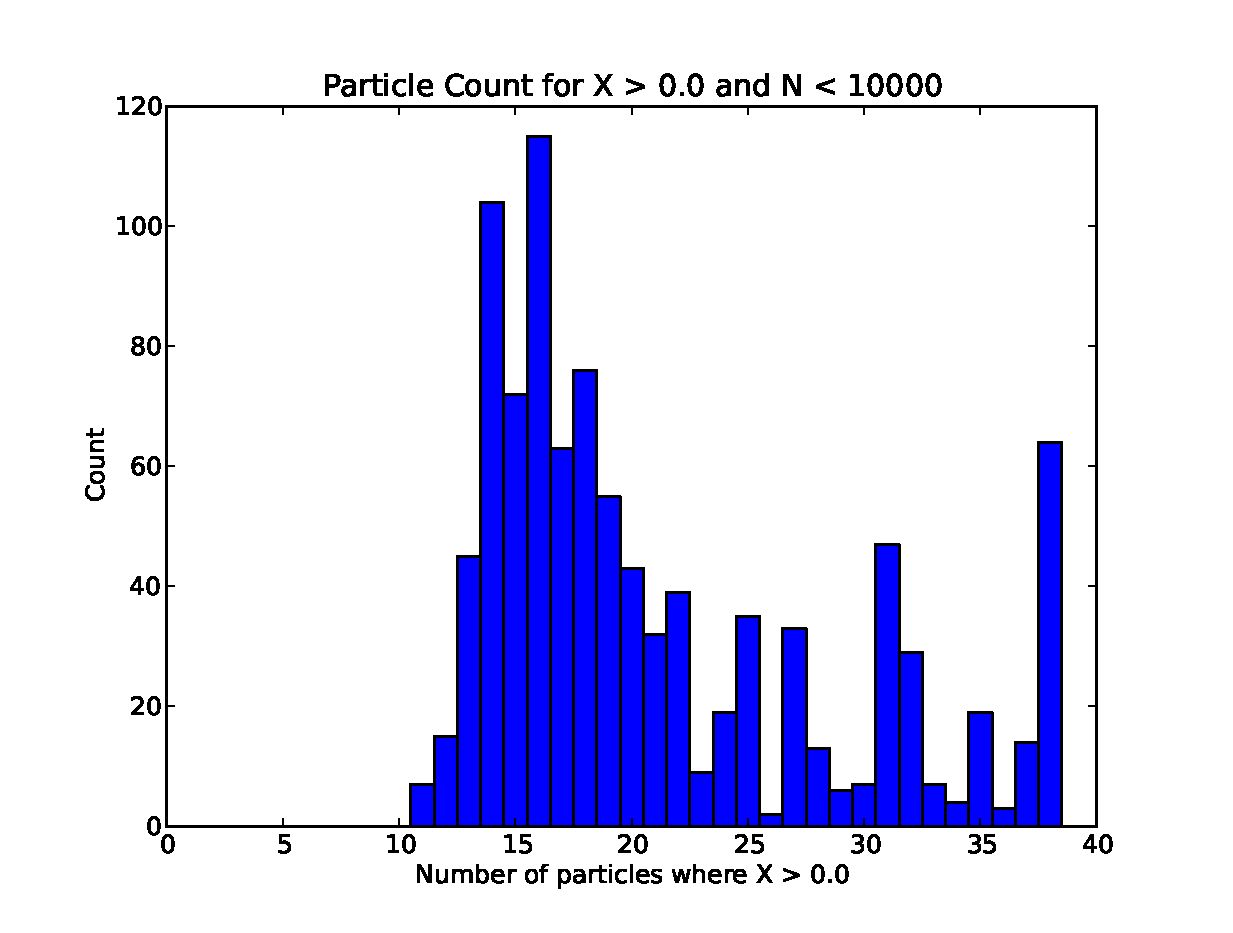
\includegraphics[width=0.5\textwidth]{images/partdist.eps}}
  \subfloat[After equilibrium steps]{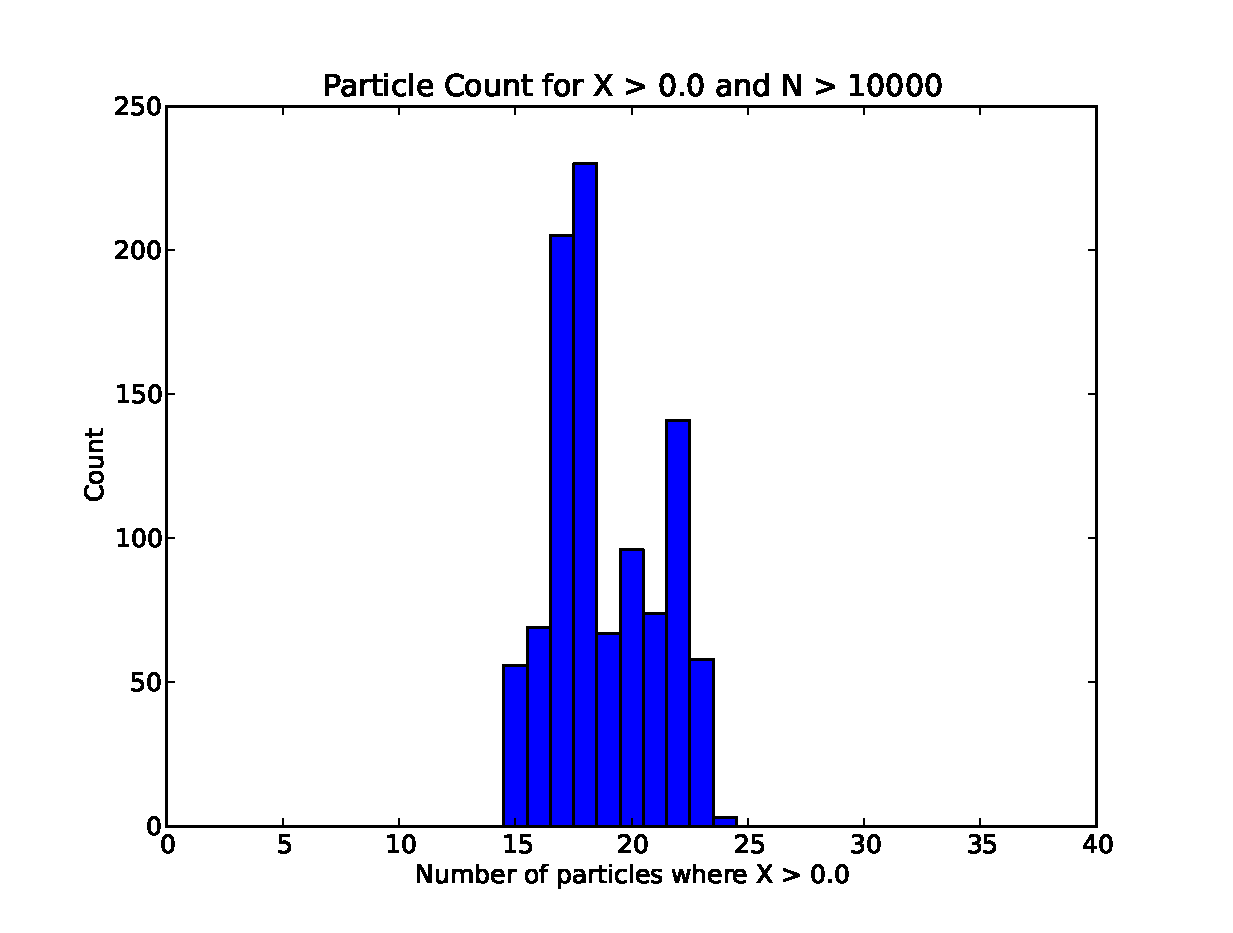
\includegraphics[width=0.5\textwidth]{images/partdisteq.eps}}
  \label{fig:partdist}
  \caption{
     Count of the number of particles placed to the right in the container, a) before and b) after 10000 equilibrium steps.
  }
\end{figure}



% ***************************************************
% END DOCUMENT
% ***************************************************

\end{document}

